\documentclass[journal]{IEEEtran}

\usepackage{iftex}
\ifXeTeX
  \usepackage{fontspec}
  \usepackage{xeCJK}
  \defaultfontfeatures{Ligatures=TeX}
  \IfFontExistsTF{TeX Gyre Termes}{\setmainfont{TeX Gyre Termes}}{}
  \IfFontExistsTF{NanumBarunGothicOTF}{%
    \setCJKmainfont[
      ItalicFont={NanumBarunGothicOTF},
      SmallCapsFont={NanumBarunGothicOTF}
    ]{NanumBarunGothicOTF}%
    \setCJKsansfont{NanumBarunGothicOTF}%
    \setCJKmonofont{NanumBarunGothicOTF}%
  }{%
    \IfFontExistsTF{Noto Sans CJK KR}{%
      \setCJKmainfont[
        ItalicFont={Noto Sans CJK KR},
        SmallCapsFont={Noto Sans CJK KR}
      ]{Noto Sans CJK KR}%
      \setCJKsansfont{Noto Sans CJK KR}%
      \setCJKmonofont{Noto Sans CJK KR}%
    }{%
      \setCJKmainfont[
        ItalicFont={Apple SD Gothic Neo},
        SmallCapsFont={Apple SD Gothic Neo}
      ]{Apple SD Gothic Neo}%
      \setCJKsansfont{Apple SD Gothic Neo}%
      \setCJKmonofont{Apple SD Gothic Neo}%
    }%
  }
  % NanumBarunGothic's CJK OpenType table does not expose U+00B7.
  % Classify it as Latin punctuation so the main Latin font renders it.
  \xeCJKDeclareCharClass{Default}{"00B7}
\else
  \PackageError{TRACE-RPG}{이 한글 원고는 XeLaTeX으로 빌드해야 합니다}{}
\fi

\usepackage{amsmath,amssymb}
\usepackage{booktabs}
\usepackage{graphicx}
\usepackage{tabularx}
\usepackage{url}
\usepackage[hidelinks]{hyperref}

\newcommand{\system}{TRACE-RPG}
\newcommand{\pendingartifact}[1]{%
  \begin{center}\fbox{\parbox{0.92\columnwidth}{\textbf{생성 근거 파일 대기 중:} #1}}\end{center}}

\title{TRACE-RPG: 감사 가능한 인터랙티브 게임 세계를 위한 이벤트 소싱 신경-기호 커밋 게이트}

\author{익명 저자%
\thanks{익명 심사를 위해 제출된 원고입니다.}}

\begin{document}
\maketitle

\begin{abstract}
대규모 언어 모델은 표현력 있는 퀘스트와 NPC 대화를 생성할 수 있지만, 유창하거나 스키마에 맞는 텍스트만으로 제안 이벤트의 실행 가능성, 권한 적합성, 정식 게임 상태와의 일관성이 성립하지는 않는다. 본 논문은 신뢰하지 않는 제안을 상태 변경으로부터 격리하는 이벤트 소싱 신경-기호 제어기 \system{}을 제안한다. 알려진 후보 필드에 대한 타입 엄격 parser, 외부에서 공급되는 행동 정책, 결정론적 상태 상대 술어가 하드 커밋 게이트를 구성하지만, 알 수 없는 candidate top-level field는 현재 거부되지 않고 무시된다. 거부된 후보에는 제한된 수리를 위한 구조화 반례를 제공할 수 있으며, 성공 후보는 변경 직전에 방어적으로 재검증한다. 할당 완전 실험 레코드는 종단 결과를 키 없는 SHA-256 무결성 체크섬과 연결하고, 의미적 리플레이는 인코딩된 전이를 재구성하며 에피소드 연속성 검사는 단절된 이력을 거부한다. 모집단 추론 대신 의도적으로 설계한 결정론적 오프라인 적합성 픽스처와 오류 주입으로 구현을 평가한다. 생성된 파일럿 산출물은 정확한 사례 수, 상태 격리 결과, 수리 경로, 지정 연산의 fault 거부 결과, 계수 검사를 보고한다. 근거 범위는 선언된 구조화 필드와 시험된 픽스처에 한정되며, 수리 생성의 provenance를 검증하거나 실시간 모델 우월성, 플레이어 효익, 감정 효능, 검색 효익, 상용 엔진 성능을 입증하지 않는다. 따라서 \system{}은 감사 가능한 트랜잭션 프로토콜과 후속 확증 게임 AI 연구를 위한 재현 가능한 기반을 제공한다.
\end{abstract}

\begin{IEEEkeywords}
게임 인공지능, 인터랙티브 내러티브, 신경-기호 시스템, 제약 생성, 이벤트 소싱, 재현성
\end{IEEEkeywords}

\section{서론}
인터랙티브 생성은 언어 과제에 그치지 않는다. 후보 이벤트가 자연스러워도 존재하지 않는 아이템을 요구하거나, 화자가 모르는 사실을 주장하거나, 금지된 퀘스트 정보를 공개하거나, 허가되지 않은 효과를 도입하거나, 퀘스트 단계를 후퇴시킬 수 있다. 실행 가능한 텍스트 환경은 그럴듯한 발화와 유효한 전이의 차이를 명시한다 \cite{S11_cote2019textworld,S12_wang2022scienceworld}. 근거 기반 대화와 개인화 퀘스트 시스템은 퀘스트, 엔터티, 그래프 맥락의 가치를 추가로 보여 주지만 \cite{S03_weir2024ontologically,S20_ashby2023personalized}, 맥락 자체가 정식 상태 변경을 승인하지는 않는다.

구조적 생성 제약은 인접한 문제를 해결한다. 문법 제약 디코딩, 언어 모델 질의 언어, 점진 파서는 생성 구조를 제한할 수 있다 \cite{S09_geng2023grammar,S10_beurerkellner2023prompting,S36_scholak2021picard}. 그러나 구문상 허용되는 이벤트도 현재 세계에 대해서는 거짓일 수 있다. 검색과 메모리는 유용한 근거를 공급할 수 있지만 \cite{S04_he2024gretriever,S05_gutierrez2024hipporag,S06_chhikara2025mem0}, 검색된 내용 역시 상태 전이의 권한 주체가 아니다.

본 논문은 이러한 관심사를 감사 가능한 트랜잭션 프로토콜로 결합한 구현인 \system{}을 제시한다. 현재 기여는 다음과 같다.
\begin{enumerate}
  \item 정식 상태, 외부 공급 행동 정책, 후보 이벤트, 실험 레코드, 게임 브리지에 대한 버전 계약;
  \item 결정론적 상태 상대 검증, 제한된 반례 유도 수리, 변경 없는 fallback, 방어적 커밋 전 검증;
  \item 콘텐츠 연결 종단 레코드, 상태 의미적 리플레이, 에피소드 연속성 검증; 그리고
  \item 엄격한 adapter 경계, 동결된 할당 키, 구별되는 종단 실패 클래스, 기술적 treatment-policy 계수를 갖춘 오프라인 harness.
\end{enumerate}
실증의 중심은 설계된 픽스처에 대한 결정론적 적합성 파일럿이다. 실시간 모델 호출, 인간 참여자, 감정 추정, 검색 실험, 실제 엔진 루프 측정은 없다. 계획된 10개 모델, 인간, 메모리, 감정, 엔진 연구는 향후 확증 확장이며 현재 결과가 아니다.

\section{관련 연구와 연구 공백}
\subsection{인터랙티브 내러티브와 게임 에이전트}
KNUDGE는 퀘스트와 엔터티 명세에 근거한 분기형 NPC 대화를 평가한다 \cite{S03_weir2024ontologically}. 지식 그래프 보조 퀘스트 생성 \cite{S20_ashby2023personalized}, 메모리--성찰--계획 에이전트 \cite{S07_park2023generative}, 학습 가능한 역할 연기 에이전트 \cite{S08_shao2023character}는 근거성과 개연성 있는 행동의 상호보완적 측면을 다룬다. 플레이어 대상 연구는 선호와 지각된 대화 품질을 평가한다 \cite{S21_akoury2023player,S22_hochreiter2026beyond}. Yin \emph{등}의 2026년 온라인 레코드는 서지 감사 당시 미래 시점의 권호가 배정되어 있어 제출 시 다시 확인해야 한다 \cite{S23_yin2026contextualized}. 2025년 프리프린트는 역할에 따른 안정성--즉흥성 trade-off를 보고하며 \cite{S02_figueiredo2025scaffolded}, 본 논문은 이를 최근 동기로만 사용한다. 이 연구들은 하드 허용 가능성을 선택적 자연스러움 및 플레이어 경험 구성개념과 분리할 필요성을 뒷받침한다.

경험 주도 콘텐츠 생성 \cite{S24_yannakakis2011experiencedriven}과 관찰자 표식 참여도 \cite{S25_melhart2020engagement}는 미래 적응 트랙의 동기가 된다. 최근 프리프린트는 vision-language model의 참여도 추론 한계를 보고한다 \cite{S26_wang2026engagement}. 따라서 감정은 비권위적 맥락으로 유지되며 현재 구현 근거에는 포함되지 않는다.

\subsection{환경과 벤치마크}
TextWorld와 ScienceWorld는 명시적인 인터랙티브 상태를 제공하며 \cite{S11_cote2019textworld,S12_wang2022scienceworld}, MineDojo는 개방형 지식 집약 embodied 과제를 추가한다 \cite{S13_fan2022minedojo}. General Video Game AI는 에이전트, 게임, 콘텐츠 트랙을 분리한다 \cite{S14_perezliebana2019gvgai}. AgentBench는 이질적인 환경의 에이전트를 연구하고 \cite{S15_liu2024agentbench}, AgentBoard는 과정 수준 진단을 추가하며 \cite{S16_ma2024agentboard}, SOTOPIA는 사회적 상호작용을 평가하고 \cite{S17_zhou2024sotopia}, BALROG는 장기 언어 및 시각 게임 추론을 평가한다 \cite{S18_paglieri2025balrog}. 자동화된 플레이 스타일 에이전트는 상호보완적인 시험 선례이지만 인간 평가를 대체하지 않는다 \cite{S19_lepelletier2022playtesting}. 이 벤치마크는 미래 평가 설계에 정보를 주지만 트랜잭션 승인 경계를 규정하지는 않는다.

\subsection{제약, 신경-기호 검증, 검색}
제약 디코더는 출력 구조를 개선한다 \cite{S09_geng2023grammar,S10_beurerkellner2023prompting,S36_scholak2021picard}. 반면 \system{}은 구조를 독립적인 상태 상대 승인의 입력 조건으로 취급한다. 현재 비아카이벌 ICCC 2026 자료와 연계된 프리프린트로 인용되는 IVIE는 가장 가까운 최근 게임 특화 신경-기호 비교 대상이다 \cite{S01_vaucher2026ivie}. 이 범위는 필요한 경계를 강조한다. 즉, 기호적 유효성은 인코딩된 목표와 술어에 대해서만 유효하다.

G-Retriever, HippoRAG, Mem0는 관련 하위 그래프 검색과 장기 메모리를 다루고 \cite{S04_he2024gretriever,S05_gutierrez2024hipporag,S06_chhikara2025mem0}, Generative Agents와 Character-LLM은 행동 메모리와 persona를 다룬다 \cite{S07_park2023generative,S08_shao2023character}. \system{}은 향후 이러한 맥락을 사용할 수 있지만 직접적인 커밋 권한은 부여하지 않는다. 검색과 시간적 메모리 효익은 여기에서 측정하지 않는다.

\subsection{감사 가능성과 재현성}
과정 지표는 중간 실패를 보존할 동기를 제공하고 \cite{S16_ma2024agentboard}, 강건한 평가는 소수 확률적 실행의 과도한 해석을 경고한다 \cite{S31_agarwal2021precipice}. 재현성과 환경 보고 지침은 동결된 산출물과 명시적 측정 경계를 뒷받침한다 \cite{S33_pineau2021reproducibility,S34_henderson2020energy}. 인간 및 LLM 평가는 구성개념, 평가자, 편향 통제를 요구하며 \cite{S27_vanderlee2019best,S28_karpinska2021perils,S29_zheng2023judging,S30_chen2024judgement}, 향후 비열등성과 참여자 분석에는 정당화된 margin과 random-effects 구조가 필요하다 \cite{S32_lakens2018equivalence,S35_barr2013random}.

제한된 novelty는 개별 구성요소의 발명이 아니라 구현된 결합이다. 승인된 36개 문헌 집합에서 보고된 시스템들은 실행 가능한 상태, 근거화, 구조 제약, 기호 검사, 검색, 메모리, 과정 측정, 재현성의 일부를 다룬다. 보고서에 기능이 없다고 해서 모든 구현에 그 기능이 없다고 추론하지 않는다. \system{}은 외부 공급 정책 경계, 상태 상대 하드 검증, 제한된 수리, 수리 이력과 연결된 종단 근거, 의미적 리플레이, 할당 완전 실패 계수를 통해 이 관심사를 함께 노출한다.

\section{문제 정의와 보장 경계}
시점 $t$에서 정식 상태는 다음과 같다.
\begin{equation}
c_t=(G_t,q_t,m_t),
\end{equation}
여기서 $G_t$는 typed world state이고, $q_t$는 외부 공급 action policy, 정식 disclosure set, quest-stage 제약을 함께 나타내며, $m_t$는 커밋된 event prefix이다. 검색, 내러티브 점수, 모델 rationale, 메모리 요약, 미래의 감정 추정은 비권위적 proposal context이다.

신뢰하지 않는 proposer가 후보 $a_t$를 출력한다. 알려진 필드에 대한 타입 엄격 parsing이 먼저 선언 스키마를 확립하지만 알 수 없는 candidate top-level field는 무시한다. validator는 다음을 반환한다.
\begin{equation}
V(c_t,a_t)=(v_{\mathrm{policy}},v_{\mathrm{pre}},v_{\mathrm{reach}},
v_{\mathrm{know}},v_{\mathrm{disc}},v_{\mathrm{quest}},E_t),
\end{equation}
여기서 $E_t$는 구조화 오류 집합이다. 상태 변경은 다음과 같다.
\begin{equation}
c_{t+1}=\begin{cases}
T(c_t,a_t), & \bigwedge_i v_i=1,\\
c_t, & \text{그 외.}
\end{cases}
\end{equation}

인코딩된 도메인의 명제는 다음과 같다. \textbf{P1 (소진 실패 불변성):} 예산 $K$까지 어떤 후보도 검증을 통과하지 못하거나 proposal/controller 실행이 commit 전에 실패하면 반환 상태는 공급된 prior state와 같다. \textbf{P2 (제한된 기록 시도):} 각 proposal 또는 repair callback이 별도로 강제된 deadline 안에 반환한다면, repair budget $K\geq0$은 최대 $K+1$개의 candidate attempt를 기록한다. 성공적인 commit은 변경 직전 수락 후보에 대한 방어적 validation을 한 번 추가한다. \textbf{P3 (효과 권한):} 수락 후보는 \texttt{ActionPolicy.allowed\_effects} 밖의 선언된 fact effect를 \texttt{CandidateAction.effects}에 포함하지 않으며, quest-stage target도 해당 policy에 의해 명시적으로 승인된다. \textbf{P4 (상태 의미적 리플레이):} 스키마와 결정론적 전이가 고정되면 수락된 trace는 명시된 terminal state를 재구성한다.

이 명제들은 올바른 정책 작성, 선언된 후보 필드로의 완전하고 충실한 추출, 결정론적 소프트웨어 버전, 단일 프로세스 파일 소유권을 가정한다. 상태 의미적 리플레이는 기록된 구조화 후보와 전이를 재검증하지만, 중간 수리의 provenance, reasoning, prompt, 확률적 생성은 재현하거나 검증하지 \emph{않는다}. 구조화 필드에서 누락된 자연어 함의는 보장 범위 밖이다.

\section{TRACE-RPG 아키텍처와 알고리즘}
\subsection{신뢰 경계와 계약}
그림~\ref{fig:architecture}는 모델 또는 recorded adapter를 canonical owner 밖에 둔다. Parser는 알려진 필드의 모호한 숫자 또는 collection type을 거부하지만 알 수 없는 candidate top-level field는 무시한다. action policy는 candidate와 별도로 공급되며 required precondition과 allowed effect를 정의한다. bridge는 commit 이후에만 versioned event를 export한다. 이는 interface를 분리하지만 상용 엔진으로의 portability를 아직 입증하지 않는다.

\begin{figure}[t]
  \centering
  \IfFileExists{../figures/fig_architecture.png}{%
    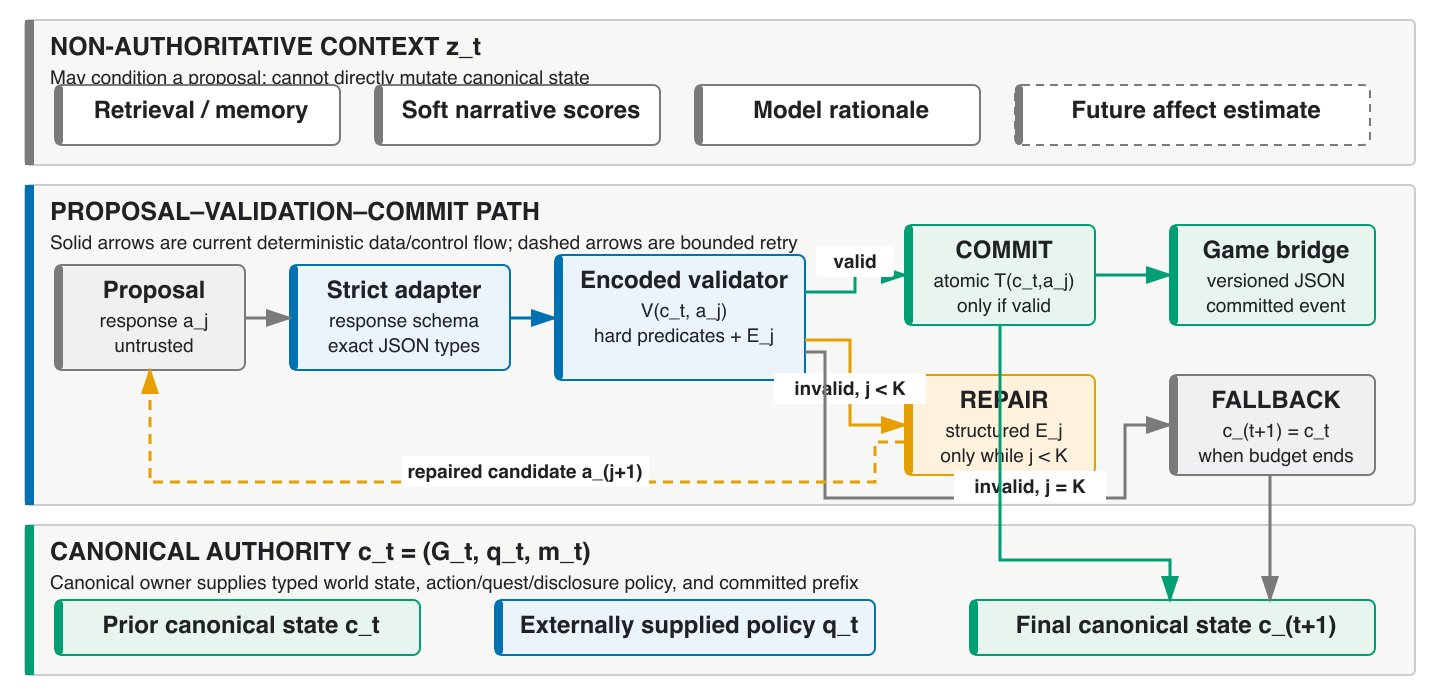
\includegraphics[width=\columnwidth]{../figures/fig_architecture.png}%
  }{\fbox{\parbox{0.9\columnwidth}{\centering 벡터 산출물 대기 중: 아키텍처와 신뢰 경계.}}}
  \caption{신뢰 경계. 검색 맥락과 생성 후보는 알려진 필드의 타입 검사와 상태 상대 validation이 완료될 때까지 비권위적이다.}
  \label{fig:architecture}
\end{figure}

\begin{table}[t]
\caption{인코딩된 Validator 경계}
\label{tab:validators}
\centering
\footnotesize
\begin{tabular}{@{}lll@{}}
\toprule
술어 & 거부 대상 & 실패 시 상태 \\
\midrule
Action policy & 알 수 없는 action/type & 변경 없음 \\
Precondition & 누락/거짓 requirement & 변경 없음 \\
Reachability & 접근 불가 object & 변경 없음 \\
NPC knowledge & 선언되지 않은 known fact & 변경 없음 \\
Disclosure & forbidden fact & 변경 없음 \\
Quest & 부적격/후퇴 stage & 변경 없음 \\
\bottomrule
\end{tabular}
\end{table}

\subsection{Validate--Repair--Commit}
제어기는 다음과 같은 추가 패키지 없는 의사코드를 실행한다. ``Record''는 in-memory trace 표현에 추가하는 것을 뜻하며, 영속 쓰기는 종단 일관성 검사 뒤에만 수행한다.

\begin{figure}[t]
\footnotesize
\begin{tabular}{@{}rl@{}}
1: & $a\leftarrow\textsc{Propose}(c)$; $j\leftarrow0$ \\
2: & \textbf{repeat} \\
3: & \quad $(ok,E)\leftarrow V(c,a)$; \textsc{Record}$(a,E)$ \\
4: & \quad \textbf{if} $ok$ \textbf{then} \\
5: & \qquad \textbf{assert} $V(c,a).ok$; \textbf{return} \textsc{Commit}$(c,a)$ \\
6: & \quad \textbf{if} $j=K$ \textbf{then return} \textsc{Fallback}$(c)$ \\
7: & \quad $a\leftarrow\textsc{Repair}(c,a,E)$; $j\leftarrow j+1$ \\
8: & \textbf{until terminal}
\end{tabular}
\caption{Validate--repair--commit 절차. 최대 $K+1$개의 candidate attempt를 기록하며, 성공 경로는 상태 변경 전 방어적 validation을 수행한다.}
\label{alg:commit}
\end{figure}

구조화 반례는 repair callback에 error code를 노출한다. repair는 상태를 직접 변경하지 않으며, 예산 소진 시 변경 없는 결정론적 fallback을 반환한다. 그림~\ref{fig:repair}는 종단 경로를 나타낸다.

\begin{figure}[t]
  \centering
  \IfFileExists{../figures/fig_repair_state_machine.png}{%
    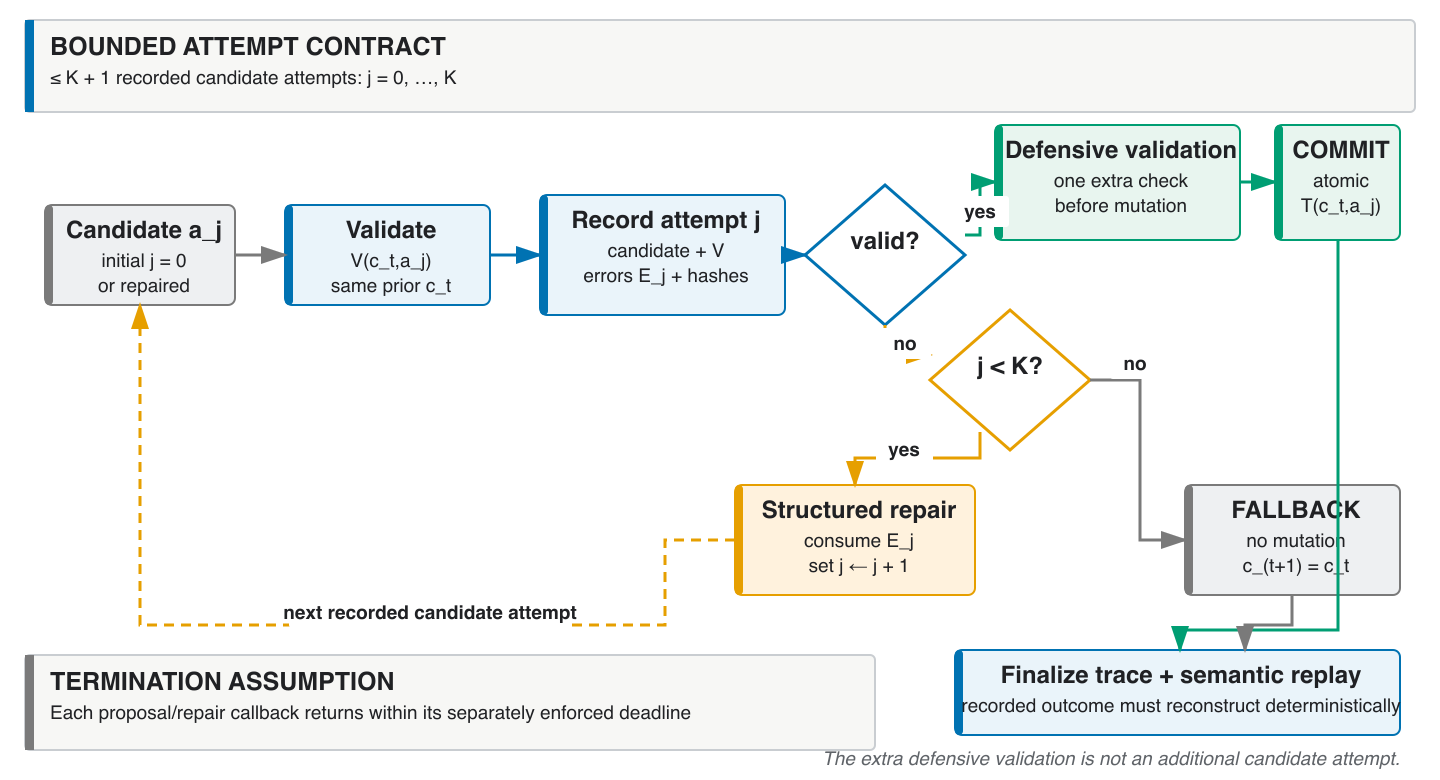
\includegraphics[width=\columnwidth]{../figures/fig_repair_state_machine.png}%
  }{\fbox{\parbox{0.9\columnwidth}{\centering 벡터 산출물 대기 중: 수리 상태 기계.}}}
  \caption{Proposal, validation, 제한된 repair, fallback, commit, replay 상태. Controller failure는 종단 상태이며 완성된 proposal trace가 없을 수 있다.}
  \label{fig:repair}
\end{figure}

\subsection{무결성, 의미적 리플레이, 계수}
각 result row는 키 없는 SHA-256 \emph{무결성 체크섬}을 가지며, proposal outcome은 추가로 trace checksum과 연결된다. 이 hash들은 우발적이거나 시험 대상인 콘텐츠 변경을 탐지하지만 signature, message-authentication code, writer identity가 아니며 콘텐츠와 checksum을 모두 다시 쓸 수 있는 행위자에 대한 보호도 아니다. 의미적 리플레이는 prior state와 기록된 모든 candidate/validation pair를 엄격히 parsing하고, final이 아닌 모든 attempt가 invalid임을 요구하며, terminal transition을 재계산하고, 명시된 final state와 비교함으로써 byte 무결성을 넘어선다. Episode replay는 인접 JSONL record 사이의 상태 연속성도 요구한다. Replay는 candidate $j+1$을 만든 repair-generation 단계를 인증하거나 다시 실행하지 않는다.

Terminal record class는 commit, symbolic fallback, adapter failure, controller failure이다. Controller-failure row는 동결된 assignment denominator에 남고 상태를 변경하지 않지만, candidate outcome이 생성되지 않았다면 완성된 proposal trace가 없어도 된다. 따라서 result completeness가 모든 terminal row의 trace 존재를 뜻하지 않는다. 실행 전 assignment key는 $(\mathrm{run},\allowbreak\mathrm{arm},\allowbreak\mathrm{scenario},\allowbreak\mathrm{seed},\allowbreak\mathrm{model},\allowbreak\mathrm{revision},\allowbreak h_{\mathrm{controller}},\allowbreak h_{\mathrm{input}},\allowbreak h_{\mathrm{prior}})$이다. 집계는 중복, 누락, 예기치 않은 key를 거부하고 symbolic, adapter, controller failure를 각각 보고한다.

\section{결정론적 오프라인 파일럿 방법}
\subsection{질문과 설계 픽스처}
파일럿은 다음을 묻는다. (PQ1) 유효 후보는 commit되고 명명된 invalid-policy 사례는 변경 없이 유지되는가? (PQ2) 작성된 repairable 및 irreparable 사례에서 rejection-only, unchanged retry, structured repair가 예상 결과를 만드는가? (PQ3) 동결된 checksum, state-semantic, linkage, continuity mutation이 지정된 검사 연산에서 거부되고, 두 번째 파일 append의 주입된 실패가 예상 pair-write rollback 검사를 작동시키는가? (PQ4) 엄격한 adapter와 assignment manifest가 할당 사례마다 정확히 하나의 분류된 terminal row를 유지하거나 fail closed하는가?

사례는 의도적으로 설계된 적합성 픽스처이며 모델 또는 게임 모집단의 표본이 아니다. 네 도메인은 validator/state isolation, repair control flow, record/trace fault injection, adapter/accounting contract이다. 반복된 결정론적 seed가 아니라 고유 사례가 기술적 denominator를 구성한다. 모든 기대값은 실행 전에 명시한다.

\subsection{측정치와 재현성}
측정치는 정확한 count이다. expected/observed validator-class agreement, rejected 또는 controller-failure 사례의 state mutation, repair arm과 repairability별 commit 및 attempt 결과, 지정된 연산에서 거부된/사전 명세된 detectable fault, replayed/committed trace, rejected/injected manifest violation을 센다. Exception class만으로 안정적인 detector layer를 식별할 수 없으므로 detector 귀속 결과는 보고하지 않는다. 의도적으로 설계된 픽스처에 $p$-value나 모집단 confidence interval을 부여하지 않는다. Recorded response의 provider-response latency는 response 수신을 조건으로 하는 과거 fixture metadata이며, local adapter timing은 end-to-end game latency가 아니다.

릴리스 패킷은 fixture 및 assignment manifest, schema, outcome/trace record를 포함한 result JSON 산출물, 환경과 코드 revision, 생성 table, checksum을 동결한다. 보고는 재현성과 측정 경계 지침을 따른다 \cite{S33_pineau2021reproducibility,S34_henderson2020energy}.

\section{파일럿 결과}
\IfFileExists{../generated/pilot_results_ko.tex}{%
  \subsection{구조 필드 게이트 적합성}
동결된 13개 게이트 fixture(유효 control 1개와 고립된 음성 fixture 12개)는 모두 사전 명세 결과와 일치했다(13/13). 구현된 오류 코드 12종이 각각 관찰됐고, 비commit 경로는 전체 정준 상태를 유지했다. 이 일치는 저자가 설계한 구조 필드 oracle에 대한 구현 적합성이며 독립 의미 판정의 정확도가 아니다.

\subsection{수리 메커니즘}
처음부터 유효하지 않은 두 case에서 rejection-only와 동일 후보 retry는 각각 0/2 commit이었다. 구조화 수리는 수리 가능 precondition case를 1회 수리 후 commit했고 수리 불가능 reachability case는 fallback하여 1/2 commit이었다. 이는 결정론적 callback의 제어 흐름 sanity check이며 LLM 수리 품질이나 sample efficiency 비교가 아니다.

\subsection{무결성, 경계, 배정 회계}
현재 명세가 검출 가능하다고 지정한 10개 fault fixture는 모두 지정된 검사 연산에서 거부됐다(10/10). 이 파일럿은 안정적인 typed detector code까지 대조하지 않으므로 detector layer 귀속을 입증하지 않는다. 별도로, 동일하게 기록된 유효 수리 앞의 무효 선행 후보를 다른 무효 후보로 치환하고 체크섬을 재계산한 알려진 provenance 경계는 예상대로 재생을 통과했다(1/1 미검출). 따라서 키 없는 체크섬을 재계산할 수 있는 작성자를 방어하지 않으며, 재생은 repair 생성 연산의 출처를 인증하지 않는다. 세 경계 sentinel---자연어 disclosure 미추출, required object의 후보·정책 동시 누락, 알 수 없는 candidate top-level field 무시---은 3/3가 의도대로 인코딩상 허용됐고 safety pass는 0건이었다. Adapter/accounting 7개 배정에서는 commit 1, 기호 fallback 1, adapter failure 5였으며, provider 응답 관측은 2/7이었다. 배정 guard 3/3가 중복·누락을 거부했다. 이 수치는 모두 합성 offline fixture의 raw count다.
%
}{%
  \pendingartifact{\texttt{../generated/pilot\_results\_ko.tex}이 아직 생성되지 않았다. 파일럿 수치나 실증 결론을 수동으로 삽입하지 않는다.}%
}

\IfFileExists{../generated/pilot_tables_ko.tex}{%
  \begin{table}[t]
\caption{결정론적 수리 arm 결과}
\label{tab:pilot-repair}
\centering\footnotesize
\begin{tabular}{@{}lccc@{}}
\toprule
Arm & 사례 & 커밋 & 수리 호출 \\
\midrule
거부 전용 & 2 & 0 & 0 \\
동일 후보 재시도 & 2 & 0 & 2 \\
구조화 수리 & 2 & 1 & 2 \\
\bottomrule
\end{tabular}
\end{table}

\begin{table}[t]
\caption{동결 파일럿 원시 집계}
\label{tab:pilot-accounting}
\centering\footnotesize
\begin{tabularx}{\columnwidth}{@{}Xrr@{}}
\toprule
검사 & 분자 & 분모 \\
\midrule
게이트 fixture 일치 & 13 & 13 \\
알려진 경계 허용$^{a}$ & 3 & 3 \\
탐지 가능 무결성 결함 거부 & 10 & 10 \\
알려진 무결성 경계 replay 허용$^{b}$ & 1 & 1 \\
Adapter 커밋 & 1 & 7 \\
기호 fallback & 1 & 7 \\
Adapter 실패 & 5 & 7 \\
Manifest guard 거부 & 3 & 3 \\
\bottomrule
\end{tabularx}
\vspace{1pt}\parbox{0.96\columnwidth}{\scriptsize $^{a}$경계 허용은 의미 추출, 정책 완결성, 알 수 없는 필드 처리의 한계를 문서화하며 safety pass가 아니다. $^{b}$Replay는 repair 생성을 인증하거나 다시 실행하지 않는다.}
\end{table}
%
}{%
  \pendingartifact{\texttt{../generated/pilot\_tables\_ko.tex}이 아직 생성되지 않았다. 결과 표는 근거 게이트 상태로 유지한다.}%
}

\begin{figure}[t]
  \centering
  \IfFileExists{../figures/fig_evidence_boundary.png}{%
    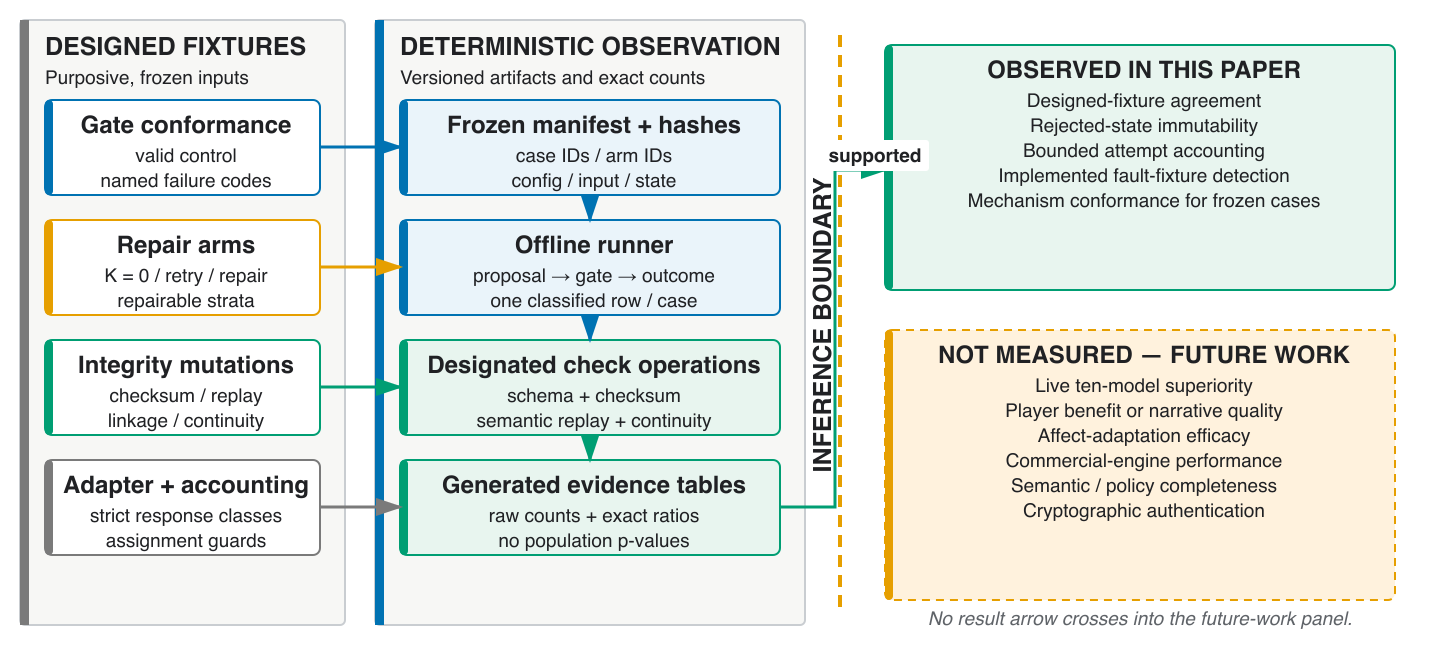
\includegraphics[width=\columnwidth]{../figures/fig_evidence_boundary.png}%
  }{\fbox{\parbox{0.9\columnwidth}{\centering 벡터 산출물 대기 중: 근거 경계와 fault-injection 흐름.}}}
  \caption{동결된 fixture에서 지정된 검사 연산과 생성 table로 이어지는 근거 경계. 수치는 생성 산출물을 통해서만 반영한다.}
  \label{fig:evidence}
\end{figure}

생성 수치와 무관하게 이 파일럿에는 live model call, participant, affect prediction, retrieval 또는 memory intervention, narrative-quality comparison, 실제 game-engine loop가 없다. 범위는 구현된 structured transition과 evidence path의 적합성이다.

\section{논의}
\subsection{확립 가능한 범위}
설계 파일럿은 동결된 사례에 대해서만 mechanism behavior를 확립할 수 있다. 인코딩된 검사가 상태를 격리하는지, bounded repair와 fallback이 선언 경로를 따르는지, 명명된 corruption이 지정된 검사 연산에서 거부되는지, assigned row가 집계를 위해 분류된 상태로 남는지를 평가한다. 거부를 안정적인 typed detector code에 귀속하지는 않는다. 이는 authoring-time validation, continuous-integration regression, recorded-adapter test, engine 이전 replay inspection에 유용하다.

이 mechanism은 policy가 올바르게 작성되었는지, 자연어 fact가 완전하게 추출되었는지, 의미적으로 unsafe한 모든 event가 declared field로 표현되었는지를 확립하지 않는다. Key 없는 hash도 writer를 인증하지 않는다. Writer는 single-process ownership을 가정하며 concurrent-writer safety는 입증되지 않았다. Versioned bridge는 interface decoupling이지 engine portability 또는 real-time performance의 근거가 아니다.

\subsection{선행연구와의 관계}
\system{}은 parsing 후 state-relative authorization을 적용하여 constrained decoder를 보완한다 \cite{S09_geng2023grammar,S10_beurerkellner2023prompting,S36_scholak2021picard}. 검색 및 메모리 구성요소에는 commit authority를 부여하지 않는다는 점에서 구별된다 \cite{S04_he2024gretriever,S05_gutierrez2024hipporag,S06_chhikara2025mem0}. 실행 가능한 환경과 benchmark를 대체하지 않고 보완한다 \cite{S11_cote2019textworld,S12_wang2022scienceworld,S15_liu2024agentbench,S18_paglieri2025balrog}. Process-linked trace는 AgentBoard가 강조한 측정 관심사를 구현하지만 \cite{S16_ma2024agentboard}, \system{}이 해당 시스템이나 다른 시스템보다 우월하다는 근거는 아니다.

\section{확증 확장}
향후 사전등록 연구는 동결된 모델 instance 10개를 선별하고 소규모 panel을 승격해 controller를 비교한다. 독립적으로 label된 semantic oracle을 사용하고, 실제 blind-retry comparator를 구현하고, attempt별 token과 latency를 기록하고, timeout 및 parse failure를 treatment-policy estimand에 유지해야 한다. Hardware/access profile마다 한 instance만 승격하면 결과는 instance 수준에 머물며 scale 또는 access effect를 식별하지 못한다 \cite{S14_perezliebana2019gvgai,S15_liu2024agentbench,S18_paglieri2025balrog,S31_agarwal2021precipice}.

Retrieval 및 memory ablation은 인코딩된 validity를 맞춘 상태에서 graph 및 conversational-memory context를 비교한다 \cite{S04_he2024gretriever,S05_gutierrez2024hipporag,S06_chhikara2025mem0}. 별도의 matched-validity human study에는 ethics review, player-qualified rater, blinding, randomized order, attention check, reliability, prospective power, 정당화된 mixed-effects analysis가 필요하다 \cite{S21_akoury2023player,S27_vanderlee2019best,S28_karpinska2021perils,S35_barr2013random}. Affect estimate는 선택적이고 비권위적으로 유지하며 validity non-inferiority margin에는 독립적 근거가 필요하다 \cite{S24_yannakakis2011experiencedriven,S25_melhart2020engagement,S26_wang2026engagement,S32_lakens2018equivalence}.

\section{타당성 위협, 윤리, 산출물 범위}
Construct validity는 declared field에 한정되며 encoded check는 누락된 의미를 발견할 수 없다. Internal validity는 독립적으로 작성된 policy expectation과 fixture leakage 부재에 의존한다. External validity는 offline text/mock case에 한정된다. Conclusion validity는 모집단 추론 없이 raw designed-case count를 보고함으로써 보호한다. Reproducibility는 고정된 software 및 artifact version에 의존한다. Security validity는 key 없는 content-integrity check와 deterministic semantic replay에 한정되며 adversarial authentication은 아니다.

파일럿은 participant 또는 personal telemetry를 처리하지 않는다. 향후 human 및 affect 연구에는 해당 review, informed consent, compensation disclosure, minimization, retention/deletion rule, opt-out이 필요하다. LLM judge를 사용하더라도 automated 및 crowd judgement 모두 calibration과 bias control이 필요하므로 보조 수단으로 유지한다 \cite{S27_vanderlee2019best,S28_karpinska2021perils,S29_zheng2023judging,S30_chen2024judgement}.

\section{결론}
\system{}은 작성된 candidate-event payload를 encoded neuro-symbolic commit gate를 통해 canonical mutation으로부터 격리하고, linked record와 state-semantic replay로 terminal outcome을 감사 가능하게 만든다. 결정론적 오프라인 파일럿은 동결된 fixture domain의 구현 mechanism에 대한 근거이지 cross-model superiority, player-experience benefit, retrieval 또는 memory effectiveness, affect efficacy, commercial-engine performance의 근거가 아니다. 이 질문들은 명시적인 확증 확장으로 남는다.

\bibliographystyle{IEEEtran}
\bibliography{../references}

\end{document}
